%%%%%%%%%%%%%%%%%%%%%%%%%%%%%%%%%%%%%%%%%%%
%%% DOCUMENT PREAMBLE %%%
\documentclass[12pt]{article}
\usepackage[T1]{fontenc}
%\usepackage{natbib}
\usepackage{url}
\usepackage[utf8x]{inputenc}
\usepackage{amsmath}
\usepackage{graphicx}
\graphicspath{{images/}}
\usepackage{parskip}
\usepackage{fancyhdr}
\usepackage{vmargin}
\usepackage{mathtools}
\usepackage{enumitem}
\setmarginsrb{2 cm}{2.5 cm}{2 cm}{2.5 cm}{1 cm}{1.5 cm}{1 cm}{1.5 cm}

\usepackage{blindtext}
\usepackage{tcolorbox}
\tcbuselibrary{minted,breakable,xparse,skins}

\usepackage[%  
    colorlinks=true,
    pdfborder={0 0 0},
    linkcolor=blue
]{hyperref}

\definecolor{bg}{gray}{0.95}
\DeclareTCBListing{mintedbox}{O{}m!O{}}{%
  breakable=true,
  listing engine=minted,
  listing only,
  minted language=#2,
  minted style=default,
  minted options={%
    linenos,
    gobble=0,
    breaklines=true,
    breakafter=,,
    fontsize=\small,
    numbersep=8pt,
    #1},
  boxsep=0pt,
  left skip=0pt,
  right skip=0pt,
  left=25pt,
  right=0pt,
  top=3pt,
  bottom=3pt,
  arc=5pt,
  leftrule=0pt,
  rightrule=0pt,
  bottomrule=2pt,
  toprule=2pt,
  colback=bg,
  colframe=orange!70,
  enhanced,
  overlay={%
    \begin{tcbclipinterior}
    \fill[orange!20!white] (frame.south west) rectangle ([xshift=20pt]frame.north west);
    \end{tcbclipinterior}},
  #3}

\title{Rapport de projet}
% Title
\author{
Yannis ELRHARBI-FLEURY \\
Sarah KERRICHE \\
Lydia AGUINI
}						
% Author
\date{25/05/2021}
% Date

\setcounter{secnumdepth}{4}

\makeatletter
\let\thetitle\@title
\let\theauthor\@author
\let\thedate\@date
\makeatother

\pagestyle{fancy}
\rhead{\thedate}
\lhead{\thetitle}
\cfoot{\thepage}
%%%%%%%%%%%%%%%%%%%%%%%%%%%%%%%%%%%%%%%%%%%%
\begin{document}
\bibliographystyle{IEEEtran}
%%%%%%%%%%%%%%%%%%%%%%%%%%%%%%%%%%%%%%%%%%%%%%%%%%%%%%%%%%%%%%%%%%%%%%%%%%%%%%%%%%%%%%%%%

\begin{titlepage}
	\centering
    \vspace*{0.5 cm}
   
\includegraphics[scale = 0.075]{Images/logo_SU.jpeg}\\[1.0 cm]	% University Logo
\begin{center}    \textsc{\Large   Sorbonne Université}\\[2.0 cm]	\end{center}% University Name
	\textsc{\Large Projet ANDROIDE : Visualisation du Paysage de valeur}\\[0.5 cm]				% Course Code
	\rule{\linewidth}{0.2 mm} \\[0.4 cm]
	{ \huge \bfseries \thetitle}\\
	\rule{\linewidth}{0.2 mm} \\[1.5 cm]
	
	\begin{minipage}{0.4\textwidth}
		\begin{flushleft} \large
		\emph{Encadrant :}\\
		Olivier SIGAUD\\
		\textbf{\Large }
			\end{flushleft}
			\end{minipage}~
			\begin{minipage}{0.4\textwidth}
            
			\begin{flushright} \large
			\emph{Étudiants :}\\
			\theauthor
		\end{flushright}
           
	\end{minipage}\\[2 cm]
	
\end{titlepage}

%%%%%%%%%%%%%%%%%%%%%%%%%%%%%%%%%%%%%%%%%%%%%%%%%%%%%%%%%%%%%%%%%%%%%%%%%%%%%%%%%%%%%%%%%
\newpage																		

\setlength{\parindent}{2ex}

\section*{Introduction}

L’apprentissage par renforcement consiste en une recherche heuristique, dans un environnement donné, d’une stratégie permettant de maximiser une récompense. \par

Dans certains environnement, cette approche est moins performante que des algorithmes évolutionnaires. De plus, il est démontré que certaines méthodes d’entraînement tirent leur efficacité de transformations de l’espace d’apprentissage. \\

Cette recherche étant propre à l’environnement, et par construction s’effectuant dans un espace en grande dimension, il est nécessaire de s’intéresser au développement d’outils permettant de mieux comprendre ce processus et d’expliquer ces phénomènes. \\

Lors de notre projet, nous avons travaillé à l’amélioration de deux outils de visualisation mis au point les années précédentes \href{https://github.com/DevMaelFranceschetti/PAnd_Swimmer/blob/master/paper_study_Swimmer.pdf}{[8]}. Ils permettent d’obtenir des aperçus du paysage de valeur autour d’un agent. \\

Lors de nos travaux, nous avons complètement réécrit le code de ces outils pour le rendre plus modulable et plus clair pour l’utilisateur. De plus, nous avons ajouté de nouvelles fonctionnalités de visualisation. \\

Dans ce rapport nous rappelons le fonctionnement des outils développés, puis détaillons notre implémentation de ceux-ci en présentant les nouvelles fonctionnalités. Nous démontrons ensuite l'intérêt de ces derniers grâce à des exemples d'utilisation, pour enfin évoquer des idées d'améliorations futures à apporter aux outils. \\

\newpage

\renewcommand*\contentsname{Table des Matières}
\tableofcontents 

\newpage
\section{Principe de fonctionnement des outils de visualisation}

Le principe de fonctionnement des outils développés les années précédentes repose sur une méthode d’échantillonnage de l’espace d’apprentissage selon des droites. \\

Les outils développés permettent d'obtenir un aperçu en deux dimensions de l'espace d'apprentissage d'un modèle, alors en grande dimension (de la taille du réseau de neurones). \\

Le premier outil, \emph{étude de gradient} \ref{gradient}, permet d'observer la trajectoire du modèle lors de son apprentissage. Le second, \emph{Vignette} \ref{vign}, permet d'observer le paysage de valeur autour du modèle. \\

La sortie de ces outils est constituée d’un ensemble de lignes de pixels. Chaque ligne est une direction tirée dans l’espace d’apprentissage, le pixel en son centre correspond au modèle à partir duquel elle est tirée. \\

La direction est ensuite échantillonnée à une fréquence entrée par l’utilisateur. La valeur d'un échantillon, quantifiée par une carte de couleur, correspond à la récompense obtenue en cette position. \\

% IMAGE d'une seule ligne
\begin{figure}[htp]
    \centering
    
\includegraphics[width=10cm]{Images/Ligne}
    \caption{Un exemple de ligne composant la sortie des outils, une droite discrétisée puis coloriée en fonction de la récompense obtenue}
    \label{fig:ligne1}
\end{figure}

Nous présentons maintenant leur principe de fonctionnement, et le format de leur sortie. \\

\subsection{Etude de gradient} \label{gradient}.

Le premier outil, \emph{étude de gradient}, permet de suivre la descente de gradient d’un modèle. \\

% IMAGE GradientStudy from above
\begin{figure}[!htp]
    \centering
    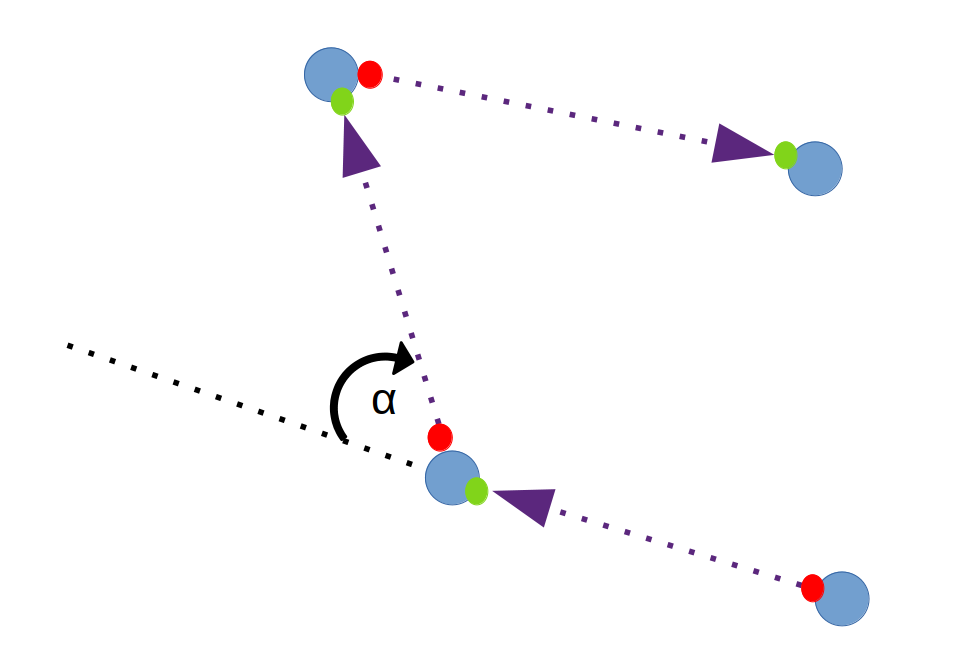
\includegraphics[width=8cm]{Images/gradientStudy_dessus}
    \caption{Descente de gradient en 2D, le modèle se déplace dans l'espace d'apprentissage en marquant un angle $\alpha$ entre deux pas.}
    \label{fig:gradientStudyAbove}
\end{figure}

Il consiste à prendre comme lignes les directions prises par la descente de gradient à chaque pas. Pour avoir une idée du déplacement effectué entre deux pas, on indique la position relative des modèles sur les droites : une pastille rouge pour la position au pas précédent, une verte pour la position au pas actuel. \\

De plus, le produit scalaire entre deux directions est représenté sur le côté droit de la sortie. L'utilisateur y lit une image du changement d'angle du modèle lors de la descente de gradient. \\

% IMAGE GradientStudy
\begin{figure}[!htp]
    \centering
    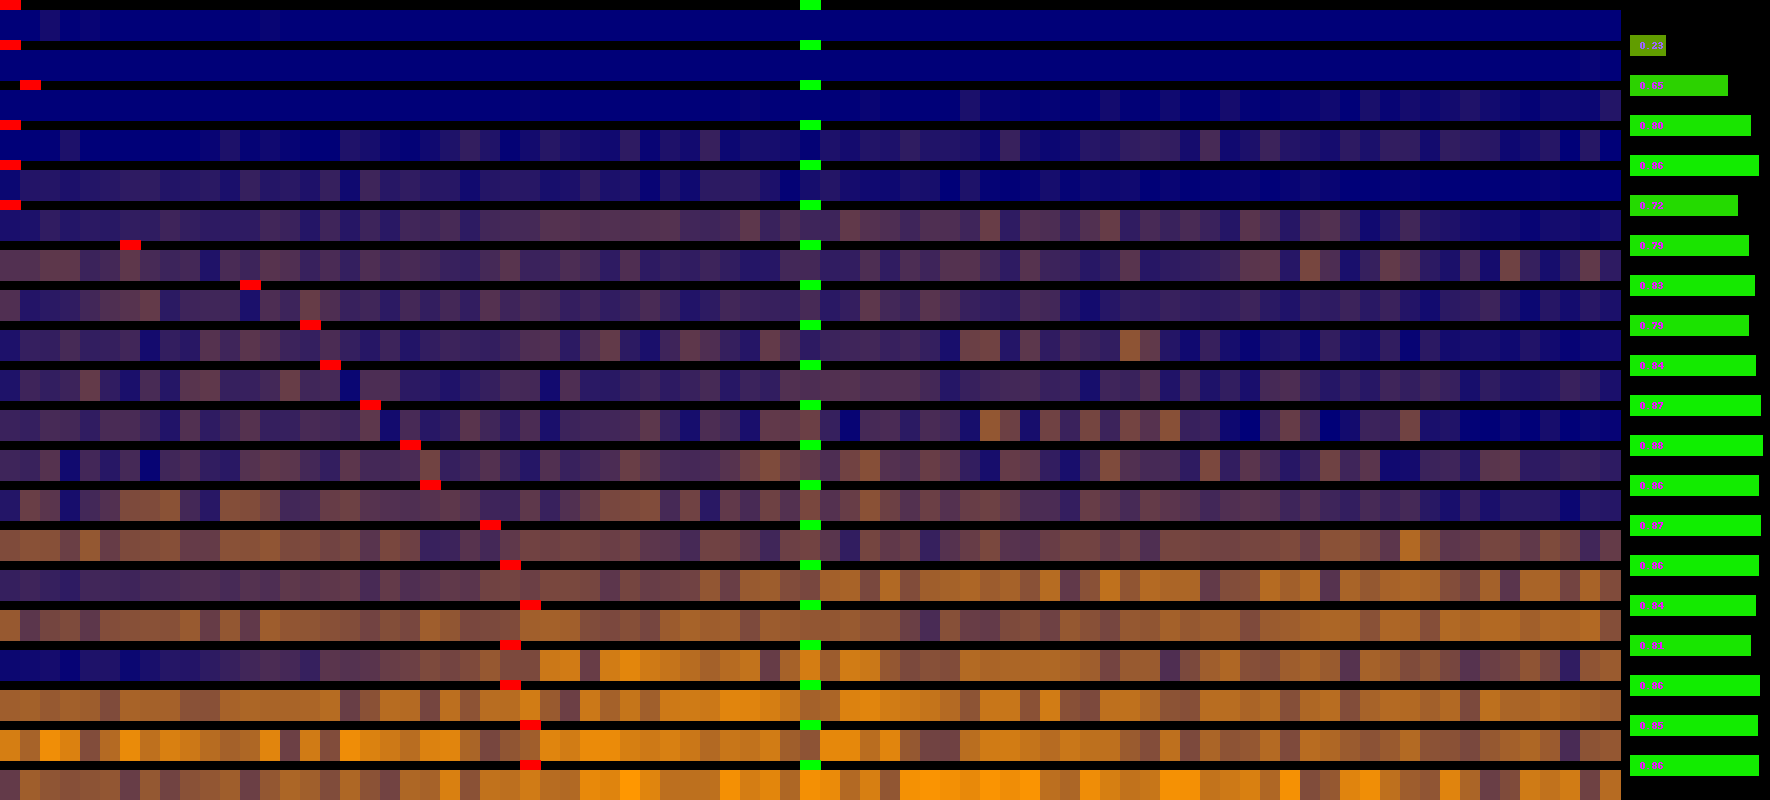
\includegraphics[width=10cm]{Images/gradientStudy}
    \caption{Un exemple de sortie de l'étude de gradient, algorithme SAC \ref{[2]}, environnement \emph{Pendulum} \href{https://pendulum.eustace.io/docs/}{[11]}  entraînement enregistré tous les 500 pas de 500 à 10.000. La sortie se lit de haut en bas, plus la récompense est grande plus la couleur est claire. De haut en bas, on observe que le modèle se déplace de moins en moins rapidement vers une zone à forte récompense. De plus, l'angle entre chaque direction est faible car le produit scalaire, indiqué sur la droite, est proche de 1. Il pourrait être intéressant d'effectuer une étude de gradient autour des premiers pas, car on observe que le changement de direction est plus le important entre le pas 500 et le pas 1.000.}
    \label{fig:gradientStudy}
\end{figure}

Ainsi, cet outil donne un aperçu en deux dimensions de la trajectoire prise par un modèle lors de son apprentissage (en n dimensions, n étant la taille du réseau de neurones). \\

\newpage
\subsection{Vignette} \label{vign}

L’outil Vignette permet d’obtenir un aperçu des alentours d’un modèle. \\

% Méthode Muller ?
Il consiste à échantillonner l’espace d’apprentissage grâce aux droites introduites précédemment. On obtient un aperçu de la boule centrée en un modèle en tirant aléatoirement à partir de celui-ci des droites partant dans des directions aléatoires.\\

Les directions tirées aléatoirement sont alors triées par ordre de proximité, dans le but de donner un meilleur aperçu des structures. Elles sont ensuite discrétisée à une certaine fréquence, ce qui permet de connaître la valeur de l'espace d'apprentissage le long de celles-ci. \\

% IMAGE Vignette principle
\begin{figure}[htp]
    \centering
    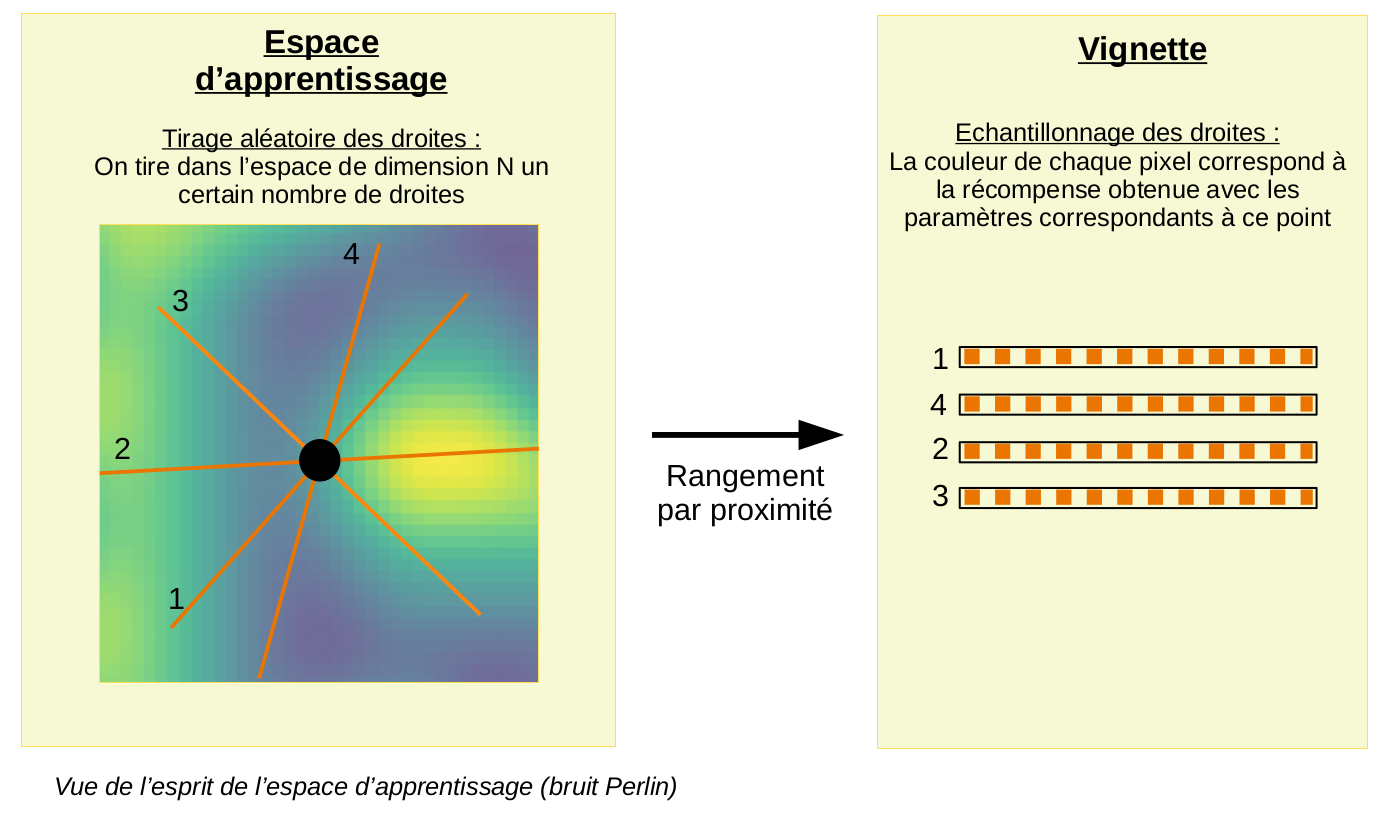
\includegraphics[width=18cm]{Images/vignetteDessin}
    \caption{Tirage des lignes de Vignette dans des directions aléatoires, centrées en un modèle initial. Elles sont ensuite groupées par proximité et sont échantillonnées pour donner un aperçu de l'espace d'apprentissage.}
    \label{fig:vignetteDessin}
\end{figure}

% IMAGE Vignette real
\begin{figure}[htp]
    \centering
    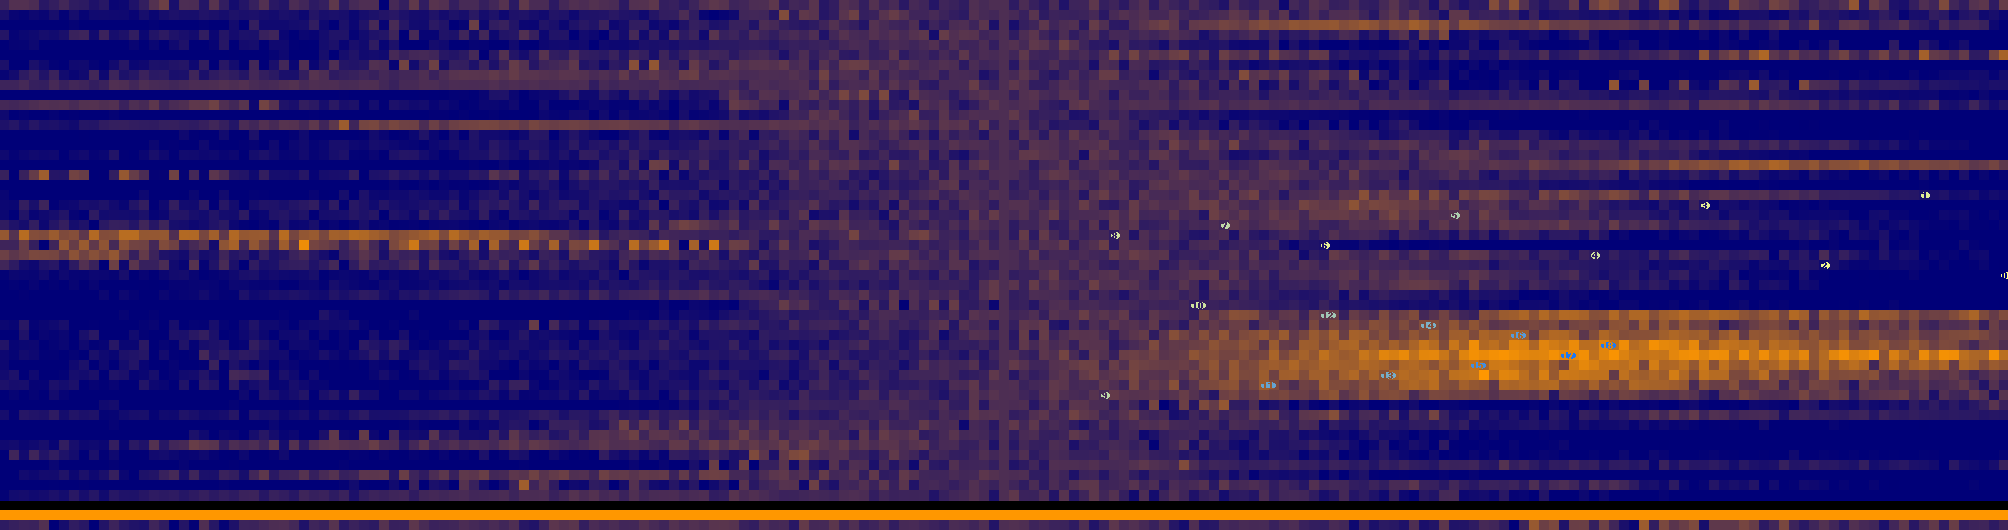
\includegraphics[width=15cm]{Images/Vignette_pendulum}
    \caption{Un exemple de sortie de \emph{Vignette}, algorithme SAC  \ref{[2]}, environnement \emph{Pendulum} entraîné pendant 5.000 pas, 50 directions tirées aléatoirement. La politique entrée est située au centre de la \emph{Vignette}. Autour du modèle, on observe un environnement bruité, de moyenne récompense. De plus, certaines zones en bordure de la boule observée sont clairement à faible récompense, tandis que deux zones à proximité offrent une meilleur récompense. On en déduit que ce sont deux zones dans lesquelles la descente de gradient est susceptible de converger.}
    \label{fig:vignettePendulum}
\end{figure}

\newpage
On obtient alors une représentation en 2D de l’espace d’apprentissage, qui était alors en grande dimension (de la taille du réseau de neurones). De plus, on observe bien la conservation des structures de l'espace d'apprentissage dans la \emph{Vignette}, avec l'apparition d'ensembles de même récompense. \\

Notons que du fait du faible nombre de directions tirées par rapport à la dimension de l'espace et de la discretisation des droites, cette représentation n’est que partielle. Il est possible que la \emph{Vignette} passe à côté de structures. \\

\section{Nouvelles fonctionnalités}

Lors de notre projet, nous avons fait le choix d'offrir à l'utilisateur toutes les fonctionnalités nécessaires pour effectuer une analyse complète du paysage de valeurs d'un environnement et d'un algorithme. \\

Ainsi, nous proposons un ensemble de fonctionnalités permettant d'aller de l'entraînement d'un modèle jusqu'à l'affichage des résultats. \\

% IMAGE Architecture projet
\begin{figure}[htp]
    \centering
    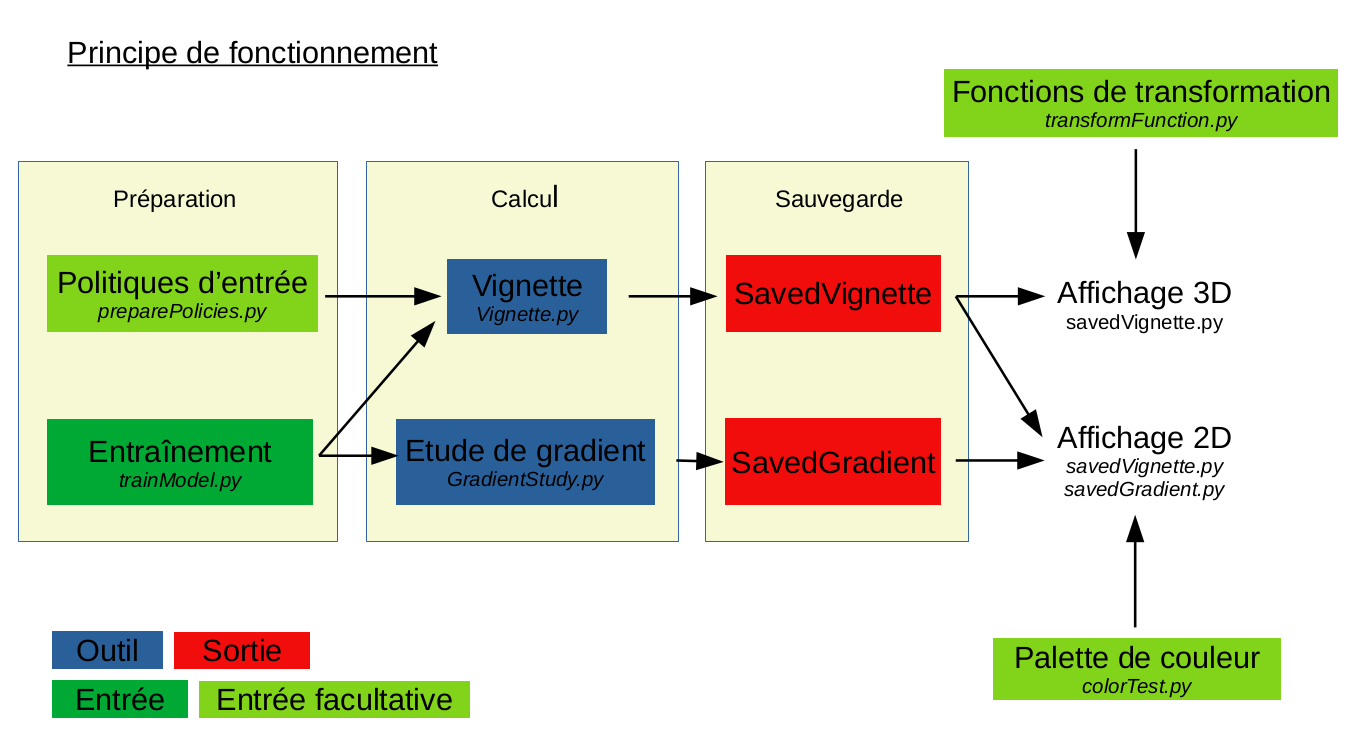
\includegraphics[width=18cm]{Images/Principe}
    \caption{Processus d'utilisation des outils}
    \label{fig:principe}
\end{figure}

\newpage
L'utilisation des outils s'effectue en trois phases : 
\begin{itemize}
	\setlength{\itemindent}{4em}
	\item préparation des entrées
	\item calcul de la \emph{Vignette} ou de l'étude de gradient
	\item sauvegarde des paysages calculés
	\item manipulation des sauvegardes pour l'affichage
\end{itemize}

Dans cette partie, nous détaillons chacune de ces phases.

\subsection*{Portage à \emph{stable-baselines-3}}

Lors de nos travaux, nous avons été contraints de réécrire le code des outils. En effet, celui-ci était écrit pour fonctionner sur un environnement particulier (\emph{Mujoco Swimmer}) sous l’algorithme TD3 \ref{[7]}. \\

Nous avons procédé à un portage vers la librairie \emph{Stable-baselines-3} \href{https://stable-baselines.readthedocs.io/en/master/ }{[12]}.
, comportant un ensemble fiable d’implémentations d’algorithmes d’apprentissage par renforcement en PyTorch \href{https://pytorch.org/  }{[13]}. Le code de cette librairie est accessible sur github et celle-ci propose une documentation détaillée de ses implémentations. \\

Ainsi, pour chacun des outils, il est possible pour l’utilisateur de changer facilement l’algorithme d’apprentissage, ses hyper-paramètres et l’environnement utilisé. \\

\subsection{Phase de préparation}

Avant toutes choses, pour fonctionner, les outils ont besoin de recevoir en entrée un modèle entraîné sous forme de réseau de neurones. \\

Grâce à leur implémentation sous \emph{stable-baselines-3 (SB3)}\href{https://stable-baselines.readthedocs.io/en/master/   }{[12]}., les outils peuvent recevoir n'importe quel réseau de neurones au format PyTorch \href{https://pytorch.org/  }{[13]}. \\

Nous proposons un exemple d'application de \emph{SB3} \href{https://stable-baselines.readthedocs.io/en/master/   }{[12]}.
 dans le fichier \emph{trainModel.py}. L'utilisateur peut alors entraîner un réseau de neurones sous l'environnement souhaité, en sauvegardant les étapes de l'apprentissage à un rythme choisi. \\

De plus, l'étude portant sur une descente de gradient, l'utilisateur peut fournir en entrée de \emph{Vignette} une liste de politiques. Il peut alors observer la position relative de chacune des politiques de la liste avec la politique centrale de la \emph{Vignette}. \\

% IMAGE politiques comparaison
\begin{figure}[htp]
    \centering
    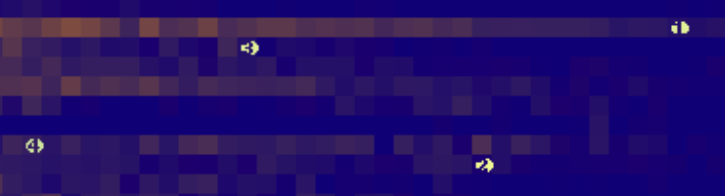
\includegraphics[width=10cm]{Images/politiques_entrees_vignette}
    \caption{Extrait d'une \emph{Vignette} affichant des politiques d'entrée}
    \label{fig:exempleEntree}
\end{figure}

Nous détaillons comment ces politiques d'entrée sont prises en compte lors du calcul de \emph{Vignette} dans la partie suivante. \\

\subsection{Phase de calcul}

\emph{L'étude de gradient} prend en entrée un ensemble de politiques, correspondant à la progression de la descente de gradient pour le modèle entraîné. Comme décrit précédemment, il calcule un suivi de la descente de gradient effectuée par le modèle. \\

% IMAGE gradientStudy Swimmer
\begin{figure}[htp]
    \centering
    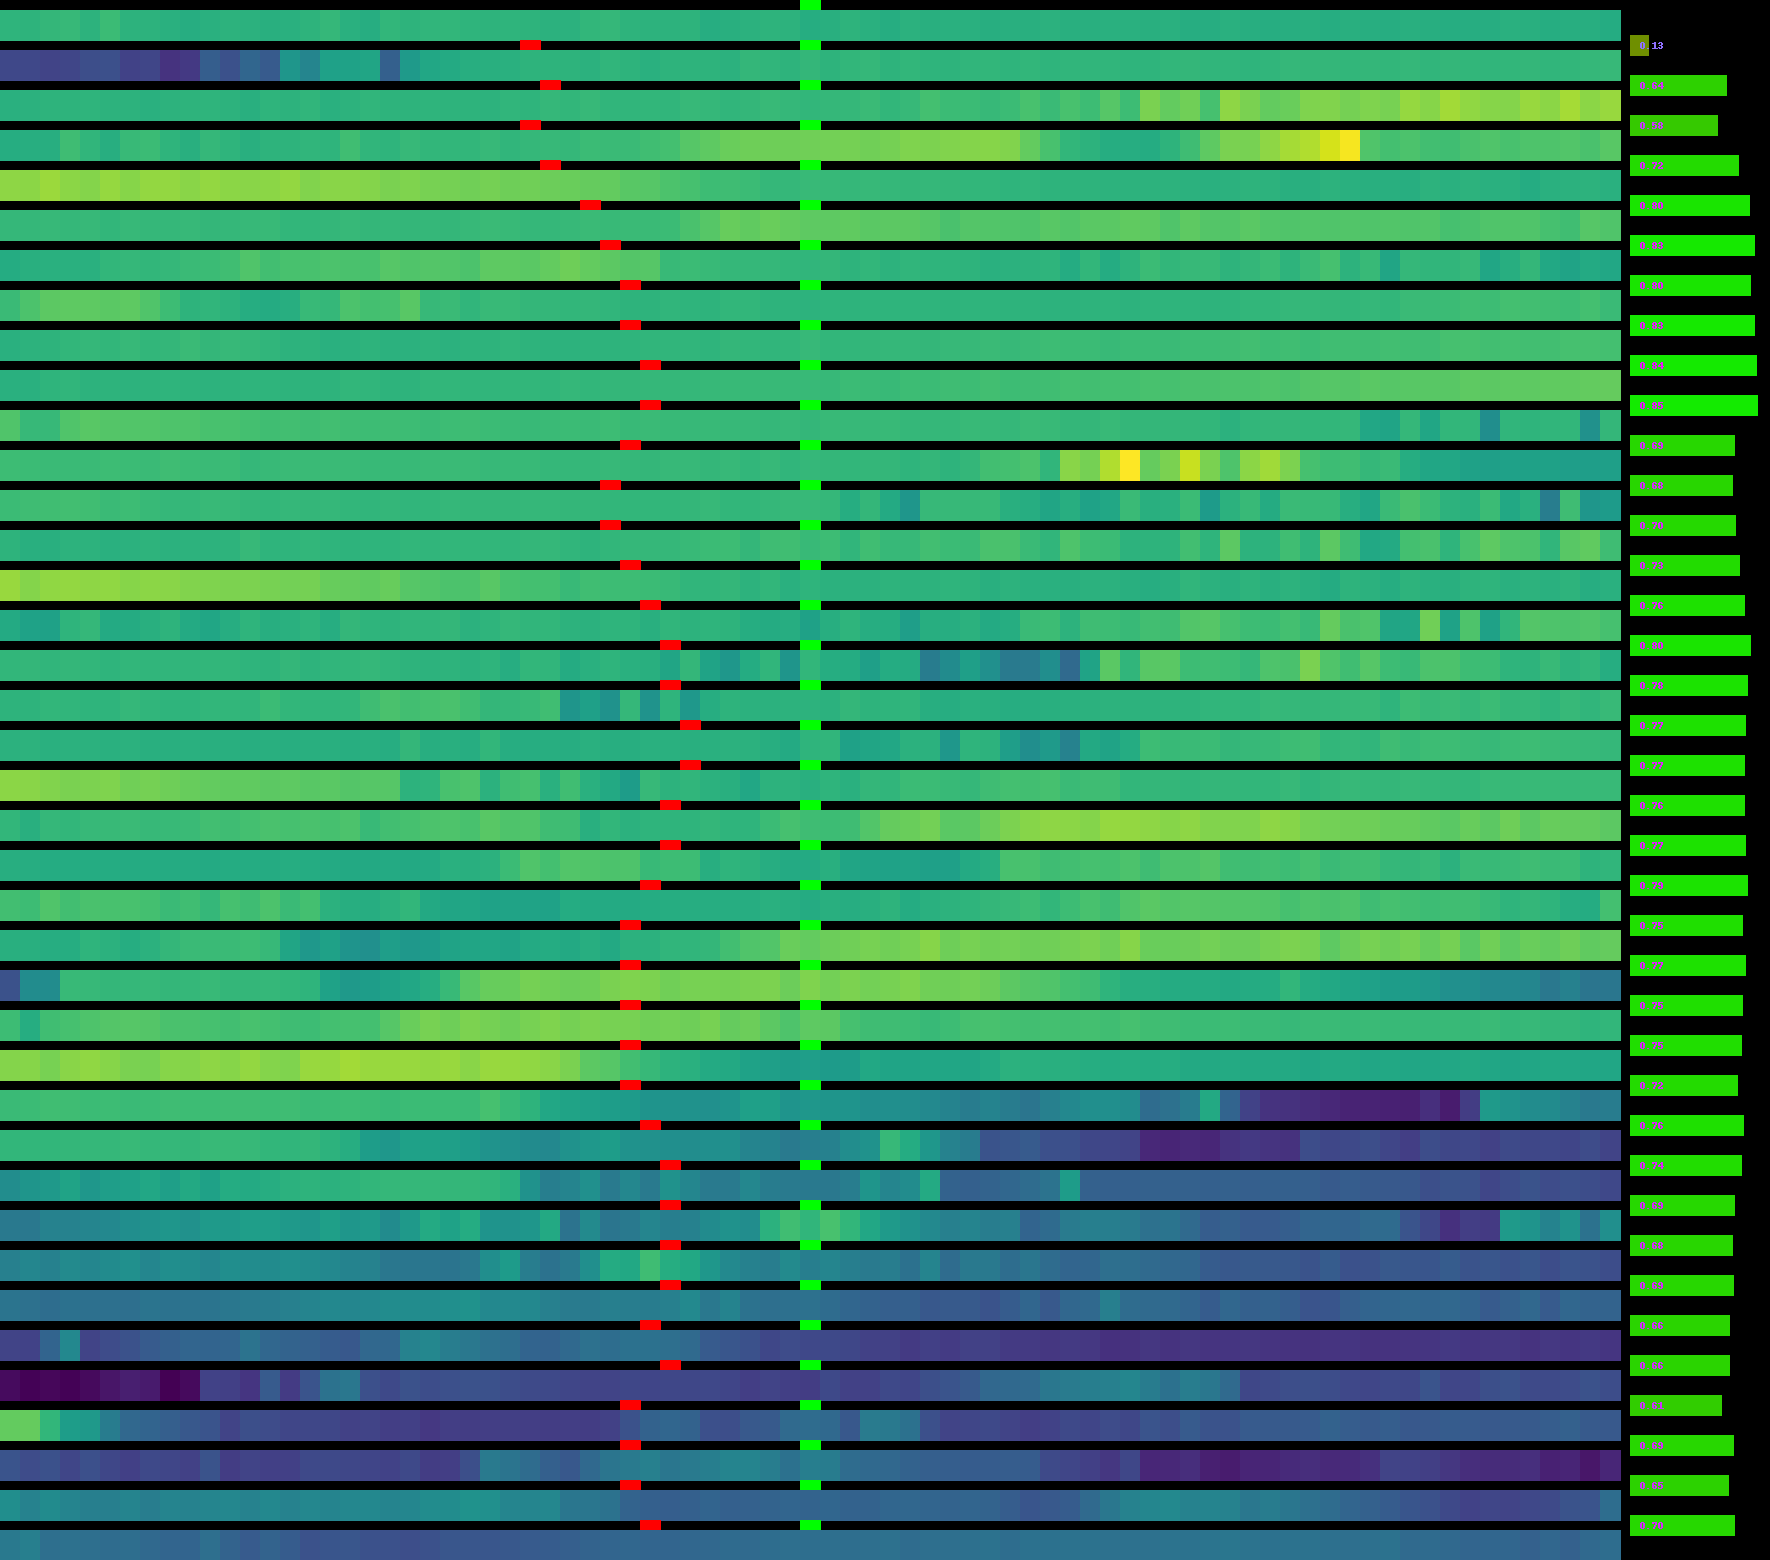
\includegraphics[width=15cm]{Images/gradientStudy_swimmer}
    \caption{Etude de gradient sur Swimmer 250 pas à 10.000 pas sauvegardé tous les 250 pas, algorithme SAC \ref{[2]}. On note tout d'abord que la normalisation des couleurs s'effectue sur les valeurs extrêmes observées, ce point sera abordé dans la section \hyperref[sec:affichage]{Phase d'affichage}. On remarque que le modèle se déplace en tâtonnant dans une zone uniforme en suivant globalement la même direction (faible angle entre chaque ligne), il finit même par réduire sa récompense. On en déduit que l'initialisation de Swimmer s'effectue dans une zone à gradient uniforme, ce qui fait partir la descente de gradient dans une mauvaise direction.}
    \label{fig:gradientStudy}
\end{figure}

Pour \emph{Vignette}, la possibilité d'entrer une liste de politiques à situer dans la sortie rajoute des étapes de calculs. Leur prise en compte s'effectue en deux étapes. \\

La première étape consiste à ajuster la fréquence d'échantillonnage des droites. \\

En effet, on rappelle que l'utilisateur donne en argument de \emph{Vignette} une fréquence d'échantillonnage. Cette fréquence correspond à la résolution de chaque ligne. Par conséquent, \emph{Vignette} dispose d'une portée limitée. On ne peut observer qu'un aperçu de la boule ayant pour centre le modèle central, et un rayon résultant de la résolution choisie. \\

Il est possible que des politiques d'entrée soient en dehors de cette boule. Nous avons donc fait le choix d'imposer une baisse automatique de la fréquence d'échantillonnage de façon à atteindre toutes les politiques. \\

\newpage
 
% IMAGE vignette portée
\begin{figure}[htp]
    \centering
    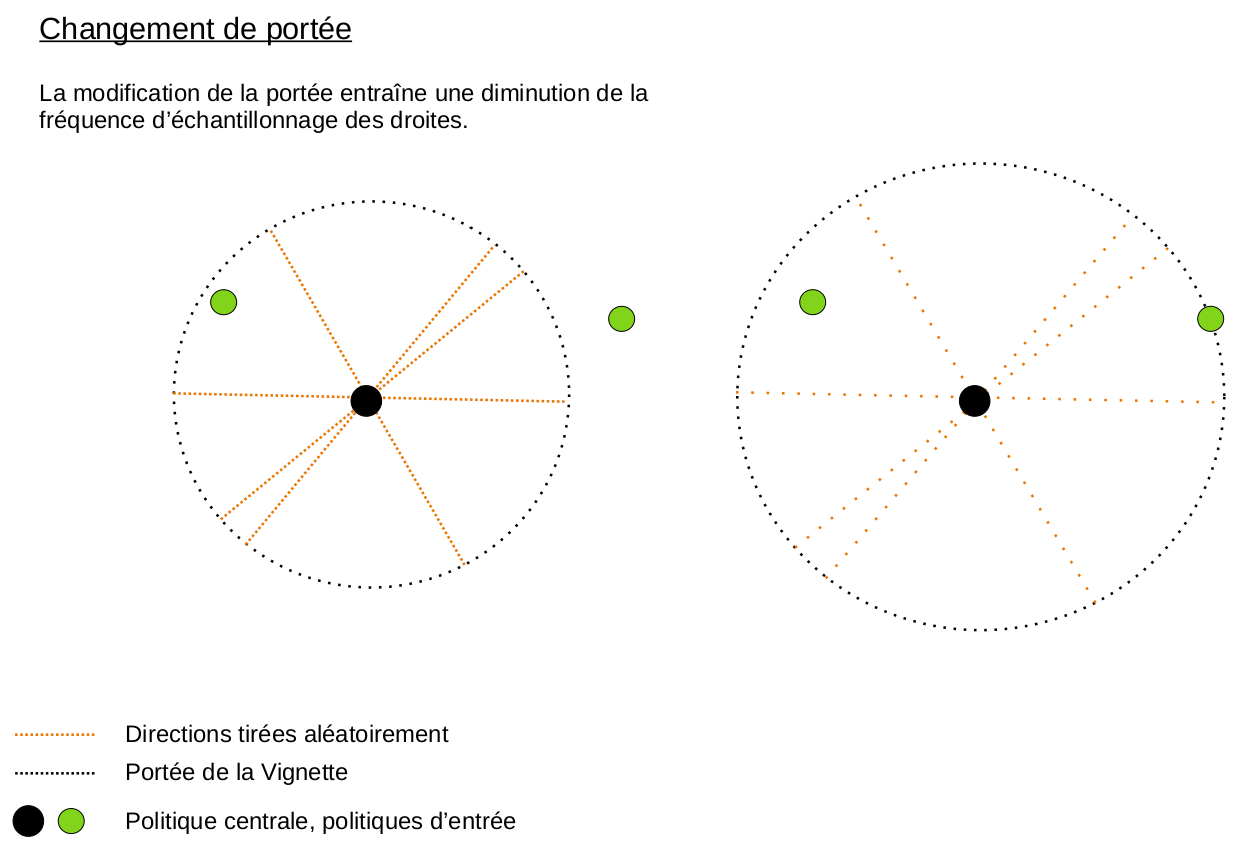
\includegraphics[width=18cm]{Images/vignette_portee1}
    \caption{Première étape : ajustement de la portée}
    \label{fig:vignettePortee}
\end{figure}

La seconde étape consiste à insérer les directions passant par les politiques d'entrée dans le résultat final. \\

Le nombre de lignes tirées (la hauteur de la Vignette) étant un paramètre de l'utilisateur, il convient de remplacer certaines de ces lignes (donc directions) par celles correspondant aux politiques d'entrée. \\

Pour que l'introduction de ces politiques bouleverse le moins possible la Vignette d'origine, on insère les directions correspondantes à la place des directions qui en étaient les plus proches. \\

% IMAGE vignette directions
\begin{figure}[htp]
    \centering
    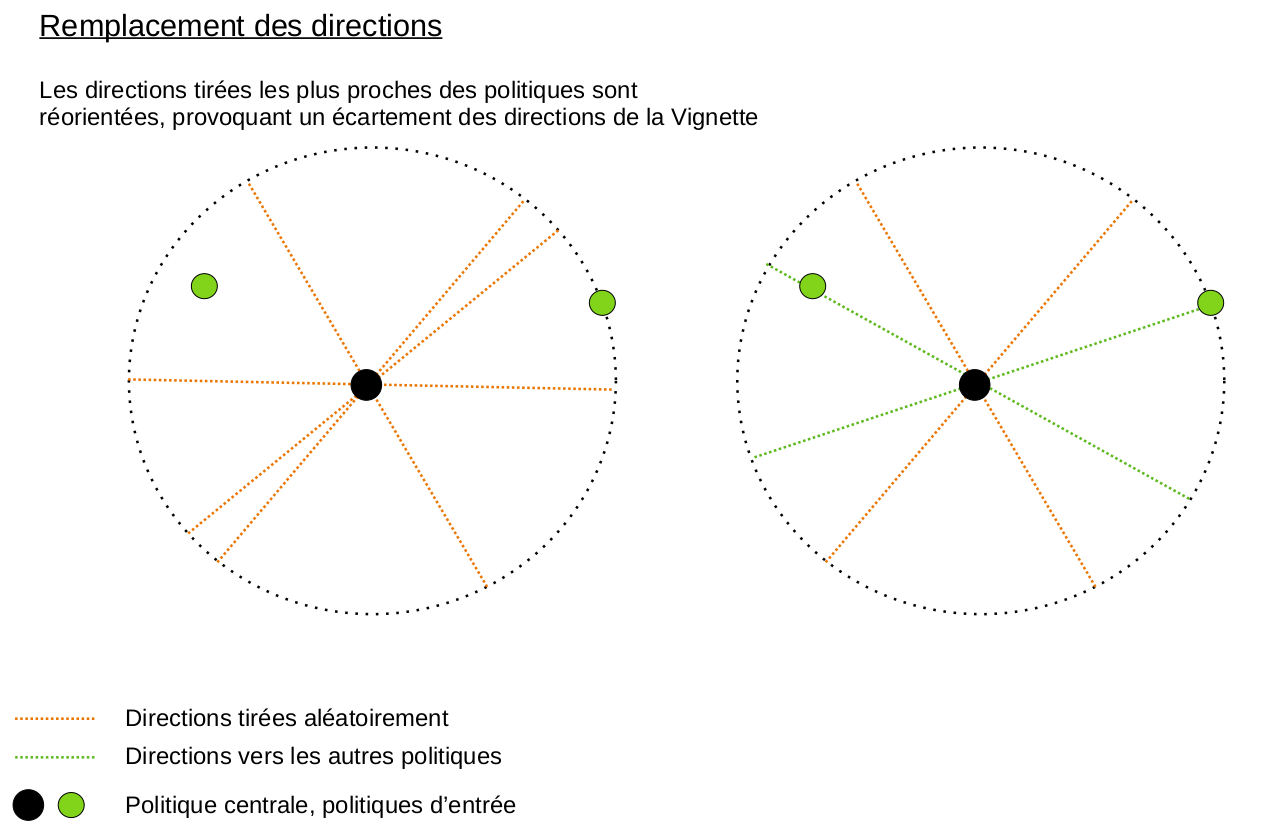
\includegraphics[width=18cm]{Images/vignette_portee2}
    \caption{Seconde étape : insertion des directions}
    \label{fig:vignettePortee}
\end{figure}

\newpage 
On constate dans l'exemple de la \hyperref[fig:vignettePortee]{figure 10} que cette étape a tendance à écarter les directions les unes des autres. \\

Cela a pour inconvénient de provoquer des discontinuités dans la détection de structures. Au contraire, l'utilisateur pourrait préférer concentrer les directions dans des faisceaux, permettant un meilleur niveau de détail autour de directions particulières. C'est un point abordé dans la partie \hyperref[sec:future]{Travaux futurs} du rapport. \\

Au lieu de choisir la direction la plus proche, une solution pourrait être de prendre la direction la plus isolée et la remplacer par la direction vers la politique. \\

C'est un problème flagrant dans notre représentation 2D simplifiée de l'espace d'apprentissage. Mais en réalité, le nombre de directions tirées est bien inférieur à la dimension de l'espace, ce qui réduit l'importance du problème. \\

\subsection{Phase de sauvegarde}

Une fois les calculs effectués, les données sont sauvegardées dans un objet de type \emph{SavedVignette} ou \emph{SavedGradient}. Chacun de ces objets garde en mémoire les directions ayant servi aux calculs, la valeur des récompenses pour chaque pixel. \\

Cette approche permet un traitement ultérieur des données si l'utilisateur le souhaite, cependant celles-ci prennent beaucoup de place en mémoire. \\

Nous utilisons une compression au format \emph{.xz} (algorithmes \emph{LZMA\href{https://fr.wikipedia.org/wiki/LZMA}{[15]}./LZMA2} \href{https://en.wikipedia.org/wiki/Lempel%E2%80%93Ziv%E2%80%93Markov_chain_algorithm}{[16]}
). Bien que ce format soit relativement lent pour la compression, il est très rapide en décompression. \\

Cela le rend idéal pour notre application : la lenteur de compression est négligeable par rapport au temps de calcul des outils (quelques secondes contre quelques heures), mais la rapidité de décompression est parfaite car l'utilisateur sera amené à fréquemment charger les résultats (pour faire des essais de modification des attributs par exemple). \\

La taille d'un fichier sauvegardé est de l'ordre de 100Mb. \\

\subsection{Phase d'affichage}
\label{sec:affichage}

Tout comme dans la version des années précédentes, nous offrons la possibilité d'afficher les résultats en tant qu'image 2D. Grâce à la fonctionnalité de sauvegarde, nous avons pu implémenter une gestion des palettes de couleur. \\

Nous avons constaté que cette gestion des couleurs était utile. En effet, elle permet aux personnes malvoyantes de régler le contraste des couleurs. De plus, certains écrans ont du mal à distinguer les faibles variations d'intensité de couleur entre les pixels. \\

L'utilisateur peut créer ses propres palettes (grâce au fichier \emph{colorTest.py}), ou utiliser des palettes de couleurs disponibles dans \emph{matplotlib}. \\

% IMAGE différentes palettes
\begin{figure}[htp]
    \centering
    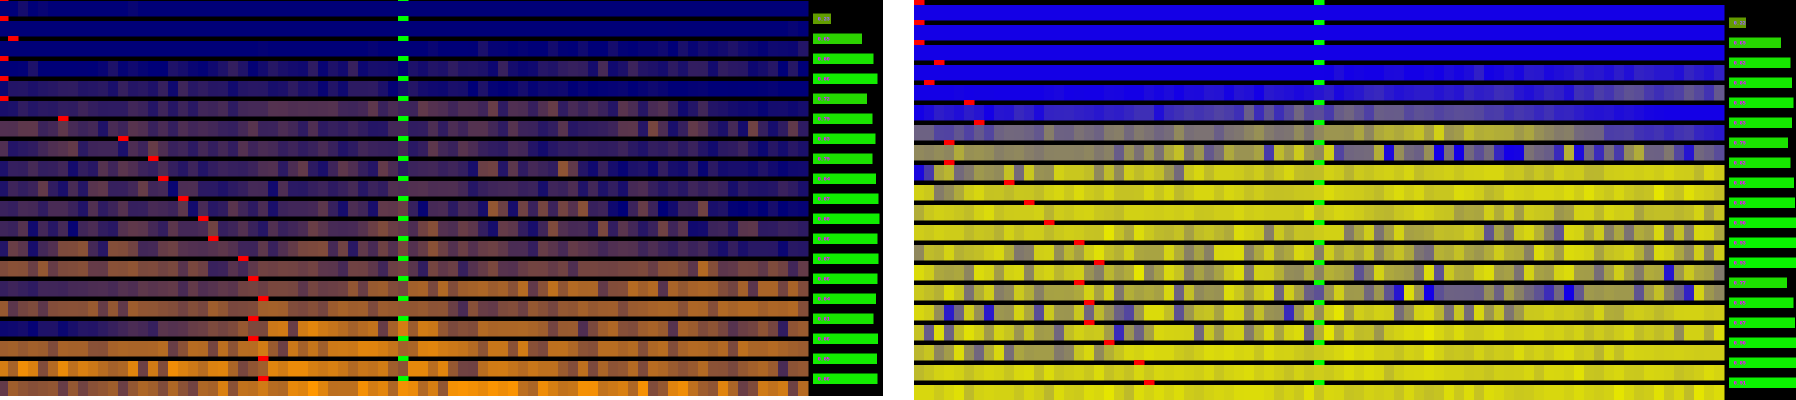
\includegraphics[width=15cm]{Images/palette}
    \caption{Différentes palettes de couleur sur la même \hyperref[fig:vignettePendulum]{\emph{Vignette}}.}
    \label{fig:palette}
\end{figure}

\newpage
La majeure partie de nos travaux a consisté à développer une visualisation en 3D de l'outil Vignette. Dans cette visualisation, chaque pixel prend pour hauteur la récompense obtenue. \\

% IMAGE Vignette 3D
\begin{figure}[htp]
    \centering
    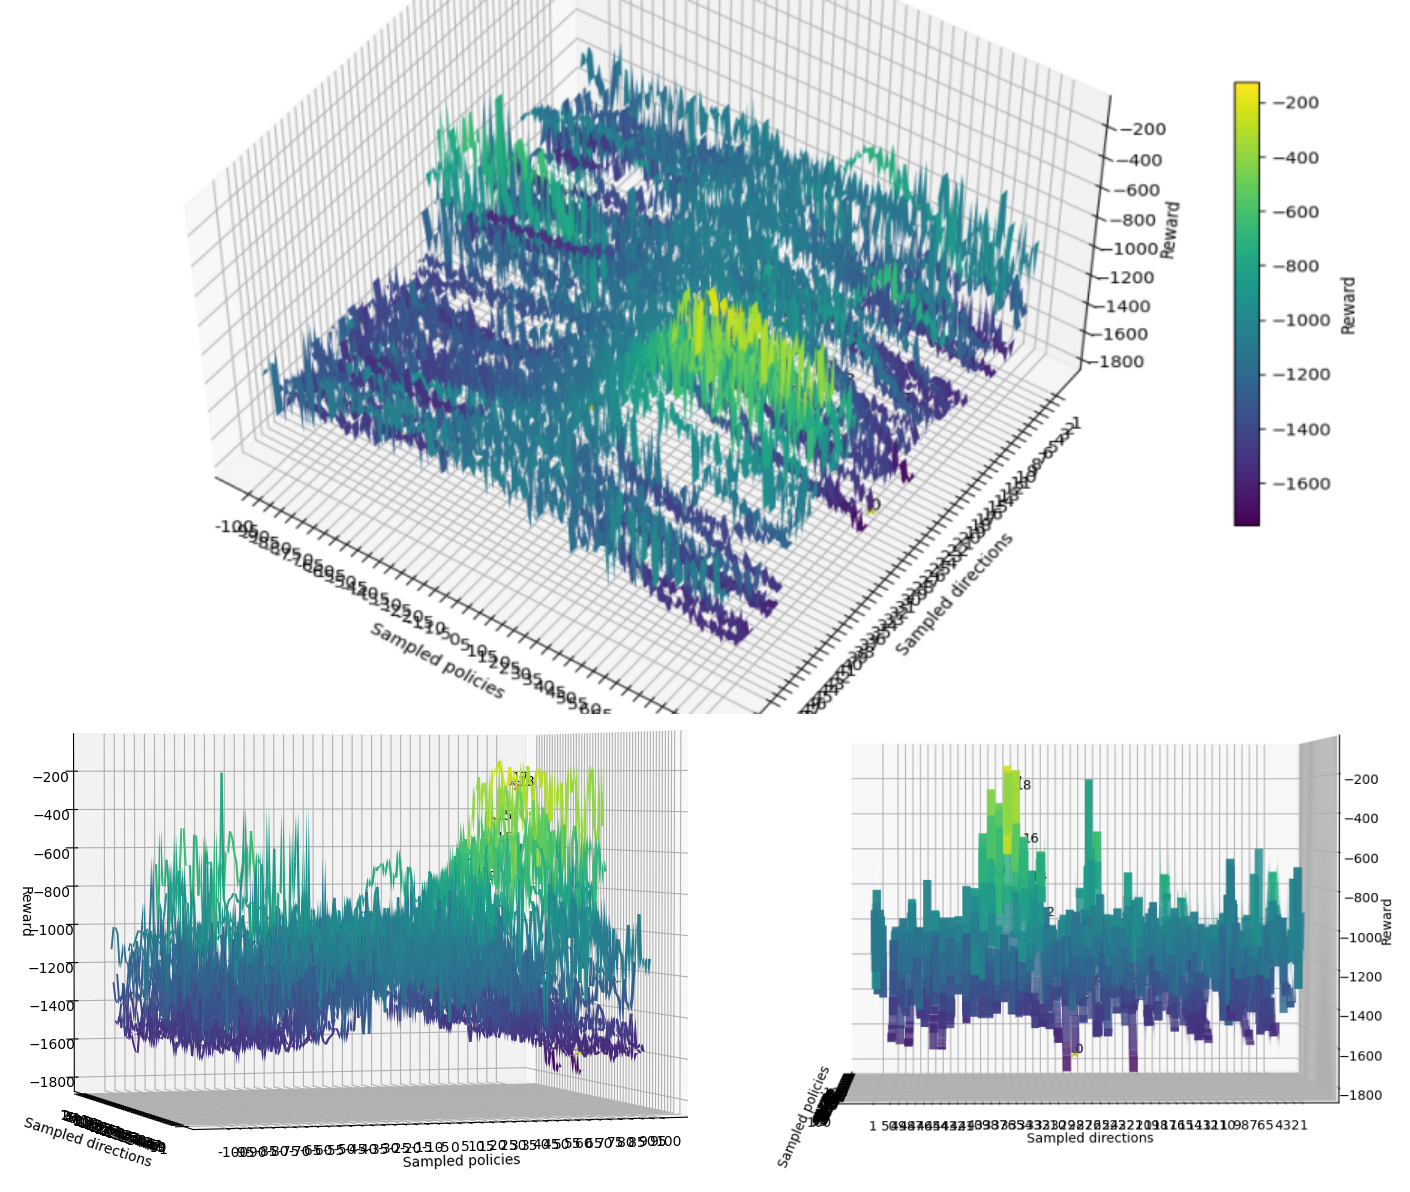
\includegraphics[width=15cm]{Images/vignette_3D}
    \caption{Vignette 3D, algorithme SAC  \ref{[2]}, environnement \emph{Pendulum} (p:\pageref{second}) entraîné pendant 5.000 pas, 50 directions tirées aléatoirement. Il est plus facile d'appréhender les structures présentes dans le paysage de valeur. Le caractère bruité du paysage est flagrant.}
    \label{fig:vignette3D}
\end{figure}

Cette visualisation contient bien les mêmes informations que la version en 2D. Cependant, elle permet une approche plus intuitive de la structure de l'espace échantillonné. \\

Sur la \hyperref[fig:vignetteDessus]{figure 13}, on remarque qu'en vue de dessus on retrouve bien la Vignette en 2D. \\

% IMAGE vue de dessus
\begin{figure}[htp]
    \centering
    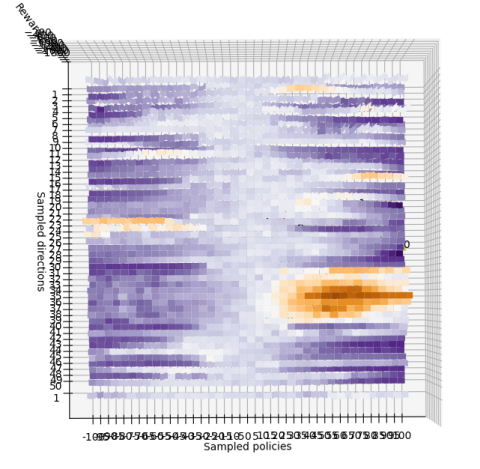
\includegraphics[width=10cm]{Images/vignette_dessus}
    \caption{Vue de dessus de la \hyperref[fig:vignette3D]{Vignette 3D}, on retrouve la \hyperref[fig:vignettePendulum]{Vignette 2D}}
    \label{fig:vignetteDessus}
\end{figure}

\newpage
Nous avons ajouté un curseur permettant de changer l'opacité des surfaces par soucis de visibilité. On peut alors plus facilement lire la position des politiques d'entrée de Vignette. \\

% IMAGE politique descente gradient + autre point de vue
\begin{figure}[htp]
    \centering
    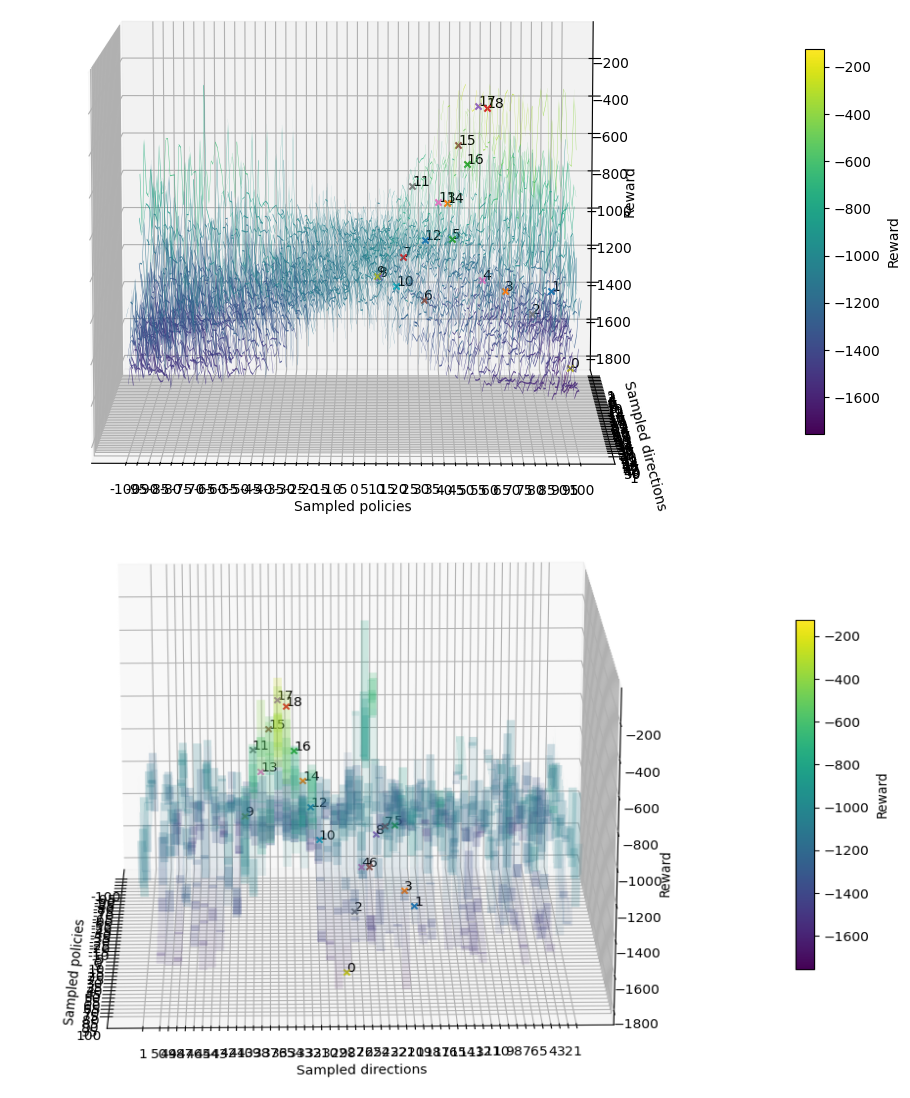
\includegraphics[width=15cm]{Images/vignette_cote}
    \caption{Vue de côté de la \hyperref[fig:vignette3D]{Vignette3D}. Les politiques en entrée de la \emph{correspondent} aux sauvegardes effectuées tous les 500 pas. On observe le processus de montée de gradient : le déplacement progressif du modèle vers une zone à forte récompense.}
    \label{fig:vignetteCote}
\end{figure}

La Vignette de la \hyperref[fig:vignetteCote]{figure 14} correspond à un entraînement de Pendulum sur 10.000 pas de temps enregistré tous les 500 pas. La politique centrale est le pas de temps n°5000, et les politiques d'entrée correspondent aux 19 autres enregistrements du n°500 au n°10000. \\

Dans l'image \hyperref[fig:vignetteCote]{vue de côté}, on observe clairement le processus de montée de gradient : \emph{Pendulum} se déplace vers des zones de plus en plus hautes (amélioration de la récompense). Cela nous donne un argument pour confirmer le bon fonctionnement de notre réécriture de \emph{Vignette} et du portage en 3D.\\

%% \subsection{Notes sur les fonctions de transformation : \emph{transformFunction}}
%% Peut être pas la place

\newpage
\subsection{Accessibilité}

D’autres améliorations ont été apportées, notamment l’ajout de barres de progression pour l’utilisateur. Il a désormais une idée plus précise de la quantité de temps restant pour les calculs. \\

De plus, le code a été clarifié et largement commenté. En utilisant le mode d'emploi, et en s'inspirant de fichiers \emph{.sh} contenant des instructions de base, l'utilisateur peut désormais rapidement prendre en main les outils. \\

Dans chaque fichier gérant les entrées et les sauvegardes des outils, nous avons laissé à la disposition de l'utilisateur des instructions types. \\

\section{Exemples d'utilisation des outils} \label{Exemples}.

% Hyper lien vers mode d'emploi ?
Les outils sont à un stade de développement assez avancé pour être utilisés dans d'autres projets, on rappelle que nous avons mis à disposition un mode d'emploi détaillant leur utilisation pas à pas. \\

\subsection{Projets utilisant Vignette}

Lors de nos travaux, nous avons bénéficié des retours d'un autre groupe P-ANDROIDE travaillant avec nos outils. \\

Le groupe d'Hector Kohler et Damien Legros \href{https://github.com/KohlerHECTOR/PANDROIDE}{[17]}. cherche à comprendre les différences de résultats donnés par deux méthodes de recherche de politique sur l'environnement \emph{Pendulum}. \\

La première méthode étudiée est la \emph{Cross entropy method} \ref{[5]}, la seconde est une méthode de descente de gradient \emph{Policy gradient}. \\

Après avoir remarqué que la distance entre politiques successives est grande dans le cas de \emph{CEM} \ref{[5]} et petite dans l'autre cas, ils ont decidé d'utiliser \emph{Vignette} pour directement observer l'espace des politiques. Ils l'ont intégré à leur code, et cela leur a permis de constater que l'initialisation des réseaux de neurones était située dans une zone plate en terme de récompense. \\

Ainsi, ils expliquent la différence de performance entre les deux méthodes par la capacité de \emph{CEM} à rapidement sortir de cette zone pour découvrir de bonnes politiques. \\

% IMAGE Hector et damien
\begin{figure}[htp]
    \centering
    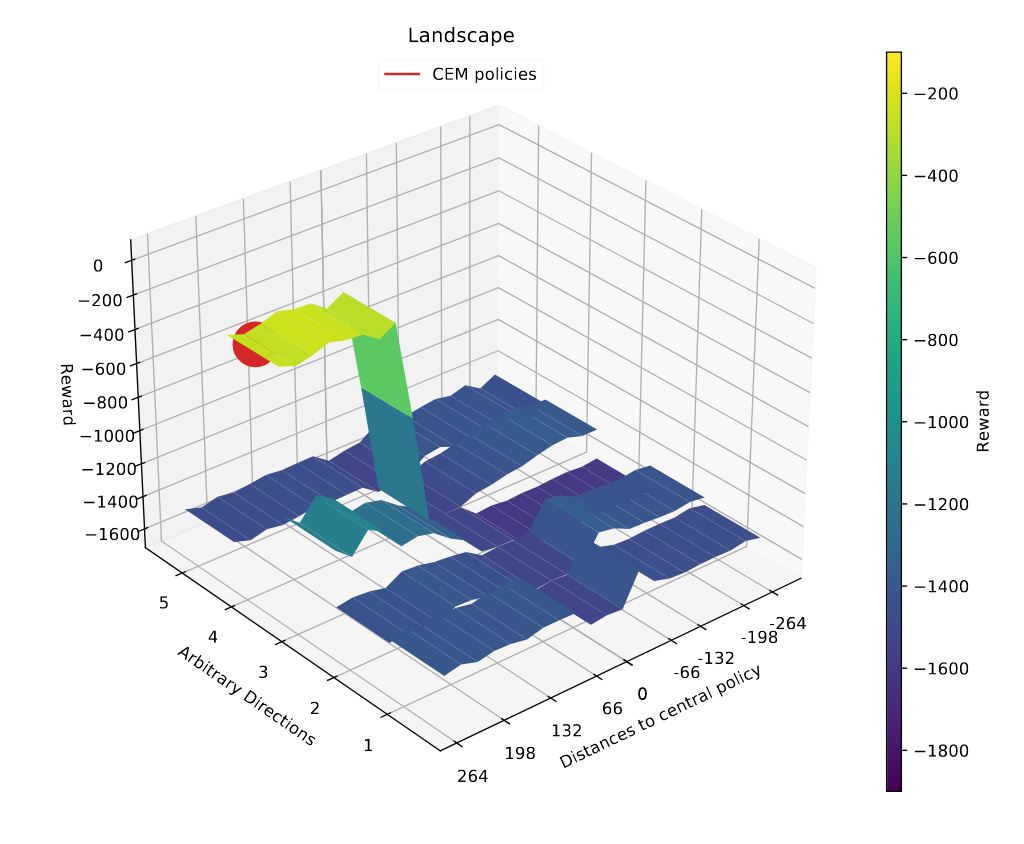
\includegraphics[width=10cm]{Images/cem_example}
    \caption{Exemple de \emph{Vignette} utilisée par le groupe de Hector Kohler et Damien Legros. \emph{Vignette} autour du point d'initialisation du réseau de neurones. On observe que la politique initiale est située dans une zone uniformément faible en terme de récompense, alors que \emph{CEM} en est éloignée dans une zone de haute récompense.}
    \label{fig:cemExample}
\end{figure}

\subsection{Régularisation de l'entropie}
%% Pas encore de données

\section{Travaux futurs}
\label{future}

Dans cette partie, nous détaillons des idées pour aller plus loin dans le développement des outils de visualisation du paysage de valeurs. \\

\subsection{Méthode des faisceaux}
% méthode des faisceaux

L'outil \emph{Vignette} permet à l'utilisateur d'obtenir un aperçu global de l'espace d'apprentissage autour d'une politique. Par ailleurs, l'outil d'\emph{étude de gradient} permet d'observer un aperçu du chemin pris par celle-ci lors de la descente de gradient. \\

Cependant, plus les sauvegardes du processus d'apprentissage sont espacées dans le temps, moins les visualisations proposées sont pertinentes. En effet, les outils ne donnent qu'un aperçu partiel de l'environnement : plus le nombre de pas entre deux politiques est grand, moins ceux-ci nous informent sur l'environnement dans lequel la descente de gradient a été effectuée. \\

Dès lors, il apparaît nécessaire de développer un nouvel outil permettant de comparer la direction globale prise par le modèle entre deux sauvegardes avec le paysage de valeur autour de la direction. \\

L'idée est de reprendre le principe de \emph{Vignette} en focalisant les directions tirées aléatoirement dans le sens de déplacement de la descente de gradient. \\

Cela revient à échantillonner un faisceau reliant un agent à un autre en trois étapes : \\

% IMAGE étapes faisceau
\begin{figure}[htp]
    \centering
    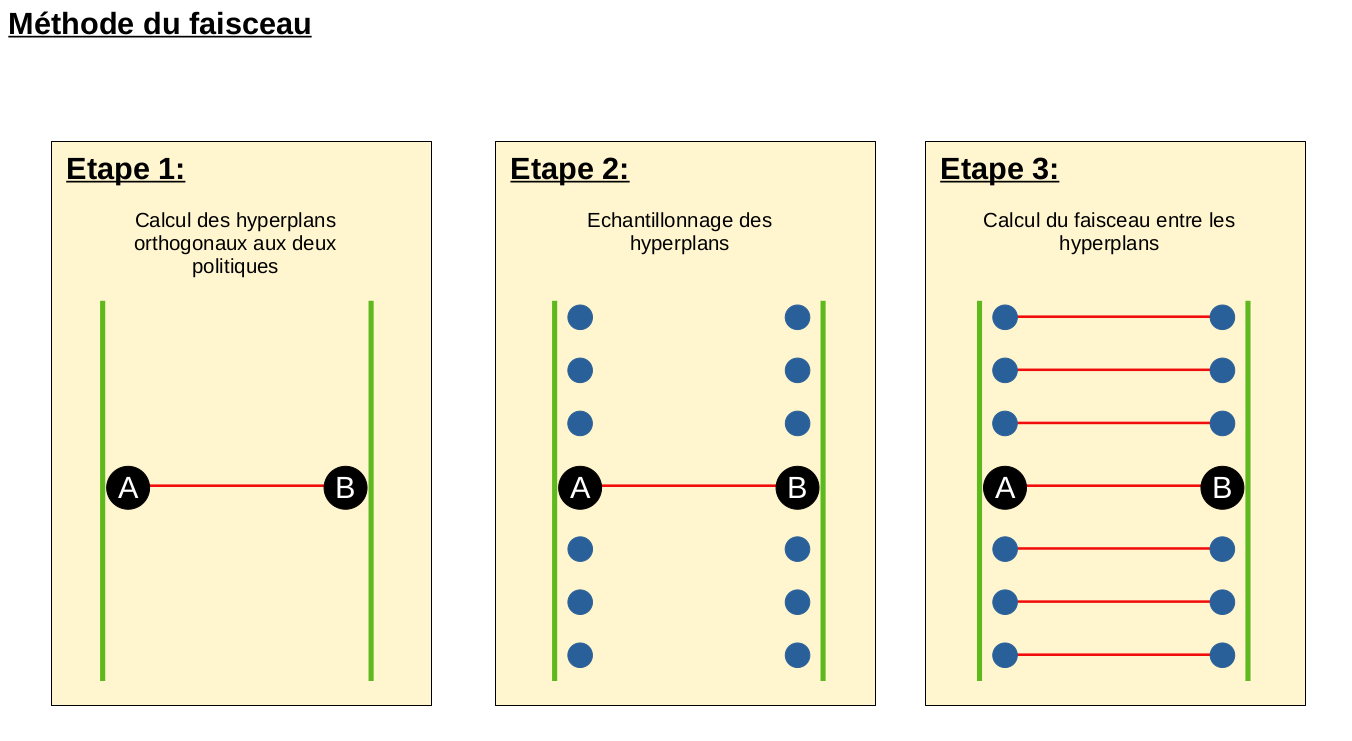
\includegraphics[width=18cm]{Images/faisceaux}
    \caption{Etapes de la méthode du faisceau}
    \label{fig:faisceaux}
\end{figure}

Dans un premier temps, on calcule la doite (direction globale) prise entre deux politiques A et B. On cherche ensuite les deux hyperplans orthogonaux à celle-ci, centrés en ces points. \\

Ensuite, on échantillonne ces hyperplans de manière uniforme pour obtenir un ensemble de politiques semblables à A et semblables à B. \\

Enfin, à chacune de ces politiques on en fait correspondre une autre sur l'autre hyperplan. On calcule les droites les reliant pour les échantillonner sur le modèle de \emph{Vignette} et \emph{étude de gradient} (voir \hyperref[fig:ligne1]{explications}). \\

% IMAGE intérêt faisceau
\begin{figure}[htp]
    \centering
    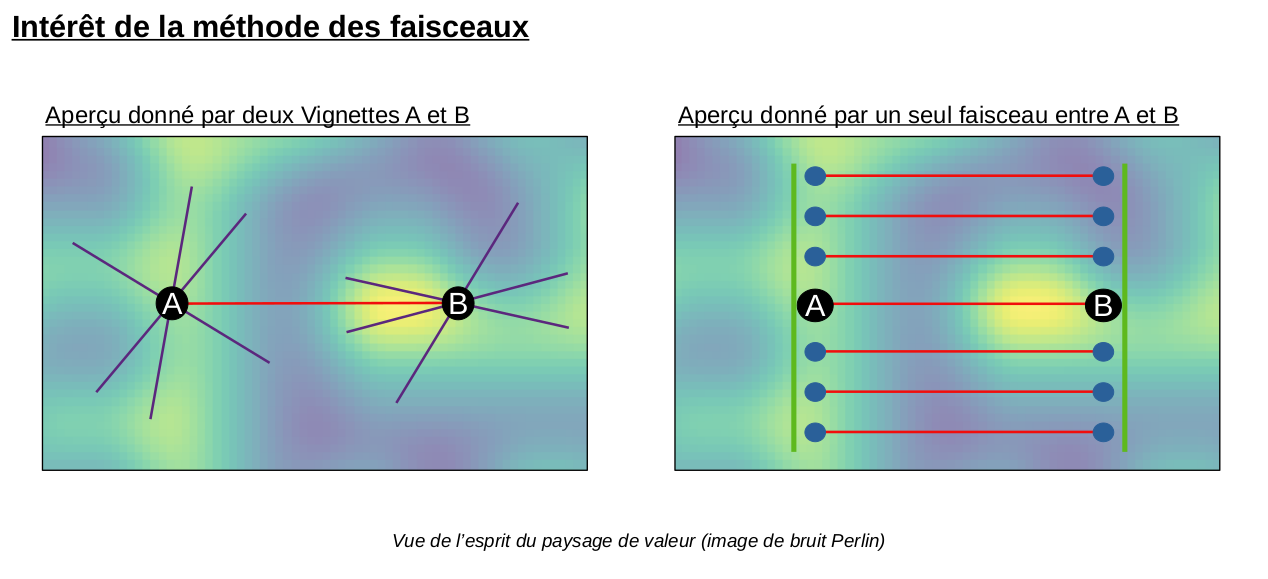
\includegraphics[width=18cm]{Images/faisceaux_interet}
    \caption{Intérêt de la méthode du faisceau : focaliser l'étude du paysage de valeur dans le sens de la descente de gradient}
    \label{fig:faisceauxInteret}
\end{figure}

On constate l'intérêt que pourrait avoir un tel outil : combiner le principe de \emph{Vignette} et de l'\emph{étude de gradient} pour mieux détecter les structures rencontrées lors de la descente de gradient. \\

\subsection{Autres fonctionnalités envisagées}

A cause du principe de généralisation, les performances des politiques ne sont pas constantes. Il est donc nécessaire de les calculer plusieurs fois pour obtenir la performance moyenne. Cela cause un problème de complexité pour le calcul de nos outils. \\

En effet, chaque pixel correspond à une politique différente. L'utilisateur est donc amené à faire un compromis entre la précision souhaitée et le temps de calcul disponible. \\

Nous proposons comme développement futur, la possibilité de calculer les outils en plusieurs passes, à différents niveaux de précision. Les résultats seraient calculés pour un faible nombre d'évaluations (donc une faible précision), permettant à l'utilisateur d'observer un aperçu des sorties pendant leur calcul. \\

De plus, nous proposons d'implémenter dans les objets \emph{SavedVignette} et \emph{SavedGradient} des méthodes permettant de segmenter l'exécution. L'utilisateur pourrait alors interrompre les calculs pour les reprendre plus tard. \\

Enfin, les échantillonnages des directions tirées dans \emph{Vignette} ou les échantillonnages des directions entre chaque pas de \emph{étude de gradient} étant indépendants entre eux, il est possible de les calculer sur plusieurs coeurs. Nous pensons que cela pourrait améliorer la vitesse d'exécution des outils. \\

\newpage
\section*{Conclusion}

Lors de ce projet, nous avons enrichi les outils développés les autres années. Après les avoir portés à la librairie \emph{stable-baselines-3}, nous les avons rendus plus faciles d'utilisation en reprenant le code à partir de zéro. \\

Il est désormais plus facile pour un utilisateur de comprendre leur principe de fonctionnement et leur architecture, notamment à l'aide du cahier des charges (\emph{user-manual}), de ce rapport et des nombreux commentaires détaillant l'exécution du code. \\

Grâce à leur implémentation sous \emph{SB3} et à l'approche objet lors de leur développement, ceux-ci sont aisément modulables et utilisables dans le cadre d'autres projets. \\

Ainsi, de futurs utilisateurs peuvent ajouter de nouvelles fonctionnalités sans avoir à modifier la structure des données. \\

Enfin, ils pourront s'inspirer de notre code pour développer de nouveaux outils de visualisation 2D ou 3D d'un espace de grande dimension, tels que la méthode des faisceaux introduite précédemment \\


\section{Réferences} \label{second}
[1] R. S. Sutton et A. G. Barto, Reinforcement learning: an introduction. Cambridge (Mass.),
Etats-Unis d’Amérique: The MIT Press, 2018. \label{[1]} \newline
[2] T. Haarnoja et al., « Soft Actor-Critic Algorithms and Applications », ArXiv181205905 Cs
Stat, janv. 2019, Consulté le: févr. 26, 2021. [En ligne]. Disponible sur:
http://arxiv.org/abs/1812.05905   \label{[2]} \newline
[3] R. S. Sutton et A. G. Barto, Reinforcement learning: an introduction. Cambridge (Mass.),
Etats-Unis d’Amérique: The MIT Press, 2018.\label{[3]} \newline
[4] O. Chapelle et M. Wu, « Gradient descent optimization of smoothed information retrieval
metrics », Inf. Retr., vol. 13, n
o 3, p. 216-235, juin 2010, doi: 10.1007/s10791-009-9110-3.\label{[4]} \newline
[5] Z. Botev, D. Kroese, R. Rubinstein, et P. L’Ecuyer, « Chapter 3. The Cross-Entropy
Method for Optimization », in Handbook of Statistics, vol. 31, 2013,p.35 59. \label{[5]} \newline
[6] P-T. De Boer, D.P Kroese, S. Mannor, and R.Y. Rubinstein. A tutorial on the cross-entropy method. Annals of Operations Research, 134(1):19–67, 2005.\label{[6]} \newline
[7] TD3 : https://www.researchgate.net/publication/341648433\_Twin-Delayed\_DDPG\_A\_Deep\_Reinforcement\_Learning\_Technique\_to\_Model\_a\_Continuous\_Movement\_of\_an\_Intelligent\_Robot\_Agent \label{[7]} \newline
[8] https://github.com/sohio92/P\_androide/blob/main/User 20manual.pdf \label{[8]} \newline
[9] https://github.com/DevMaelFranceschetti/PAnd\_Swimmer/blob/master/paper\_study\_Swimmer.pdf. \label{[9]} \newline
[10] https://github.com/DevMaelFranceschetti/PAnd\_Swimmer \label{[10]}\newline
[11] https://pendulum.eustace.io/docs/ \label{[11]}\newline
[12] https://stable-baselines.readthedocs.io/en/master/  \label{[12]}\newline
[13] http://www.mujoco.org/ \label{[13]}\newline
[14] https://pytorch.org/  \label {[14]}\newline
[15] https://fr.wikipedia.org/wiki/LZMA \label{[15]}\newline
[17] https://github.com/KohlerHECTOR/PANDROIDE \label{[17]}\newline 
[16] https://en.wikipedia.org/wiki/Lempel\%E2\%80\%93Ziv\%E2\%80\%93Markov\_chain\_algorithm \label{[16]} \newline

\end{document}
